\section{Recipe}\label{sec:recipe}
Looking into earlier projects developed using UPPAAL, an item being produced is often implemented as a sequence of actions, which must be taken in order to complete the item. Therefore items are often referred to as recipes. We will do the same from this point on. 

There are of course different ways of implementing a recipe. The simplest variant is a list of actions, which must be performed linearly. However, we find it more flexible to implement a recipe as a dependency graph. This is because we often do not care for the precise sequence of actions, just that some actions are performed before others. This is easily described using a dependency graph as seen in \cref{fig:dependency-graph}. This recipe describes that it needs to be hammered and screwed before it is packaged. Yet, it cares not in which order the hammering and screwing takes place. 

\begin{figure}[h]
\centering
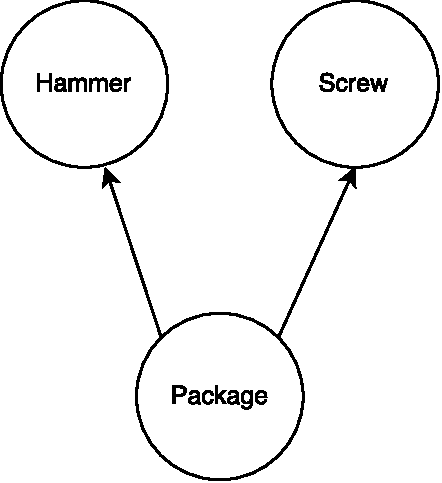
\includegraphics[width=0.3\textwidth]{dependencygraph.pdf}
\caption{Dependency graph describing order of actions}
\label{fig:dependency-graph}
\end{figure}

We know that in some real life systems, a single item may be created through the aggregation of parts, which are individually produced. To escape this complexity, we only consider items, whose production is never distributed. That is, the production of an item starts at one single point and ends at another point never splitting up. As we represent recipes as dependency graphs, it also means that the same work can not be applied on a recipe several times, as this would produce cycles in graph. 

In the following we describe how we handle recipes in our model through the use of the \emph{Recipe} and \emph{RecipeQueue} templates.


\subsection{Recipe}\label{subs:recipe}
It is possible to construct a functional dependency graph in UPPAAL using the graphical tools,  creating a new template for each new recipe type. However, as will be revealed in \cref{ch:configuration}, we wish to be able to instantiate a system and its recipes through python, instead of writing directly in UPPAAL. This requires that we edit the XML file in which our model is described. Having to generate a new template from scratch for each recipe type, would be very cumbersome. Instead we create a single recipe template that, depending on its instantiating parameters, functions according to a specific functional dependency graph. Thus we only have to generate code for instantiating templates.

Our recipe template can be seen in \cref{fig:recipe}. To describe the underlying functional dependency graph, the template is instantiated with an array of nodes. The \emph{Node} struct is shown in \cref{code:Node}. This reveals that each node knows what type of work it represents, the number of parents it has, its children's indexes in the node array and the number of children. Node A is parent of node B if B depends on A and the other way around for children. In addition a recipe is also instantiated with a unique id, the id of the module it begins at, as well as the direction it enters this module from. 

\lstinputlisting[language=C, caption=Node struct, captionpos = b, label={code:Node}, float]{codeRelated/UPPAAL/node.txt}

When a recipe begins processing, it is placed onto its start module, and we find the ids of nodes, which do not depend on any other node. The ids of these are placed into the local \emph{current\_nodes} array, and represent what works can be performed on the recipe. After this, the recipe is moved along the factory. Each time it meets a module, where it wishes to have work performed, it will handshake on its own private channel with the module to identify itself. Afterwards it will synchronize with the module again on one of the allowed \emph{work} channels. A work channel can be synchronized on, if one of the nodes in the \emph{current\_nodes} array, represent the work type corresponding to that work channel. This check is done by the \emph{is\_callable} function.

Before going back to the \emph{InProgress} location, a call to \emph{update\_current\_nodes} is made. The code of this function can be seen in \cref{code:updatecurrentnodes}. It will first collect all current nodes in the \emph{new\_nodes} array, except for \emph{called\_node}, as this is the node just worked on. It then runs over each of \emph{called\_node}'s children to decrement their \emph{number\_of\_parents} field by 1. If this field reaches 0, it means that the node no longer has any dependencies and can be worked on. Because of this it is added to the \emph{new\_nodes} array. Once all children have been updated, the contents of \emph{new\_nodes} are used to update \emph{current\_nodes}.  

\lstinputlisting[language=C, caption={The update\_current\_nodes function}, captionpos = b, label={code:updatecurrentnodes}, float]{codeRelated/UPPAAL/updatecurrentnodes.txt}

After the call to \emph{update\_current\_nodes} is finished, we call \emph{no\_more\_nodes}. This will set the local \emph{done} boolean to \emph{True}, if \emph{current\_nodes} nodes is empty. This means that the recipe can not be worked on any further and may be removed.

\subsection{RecipeQueue}\label{subs:recipequeue}

\begin{figure}[h]
\centering
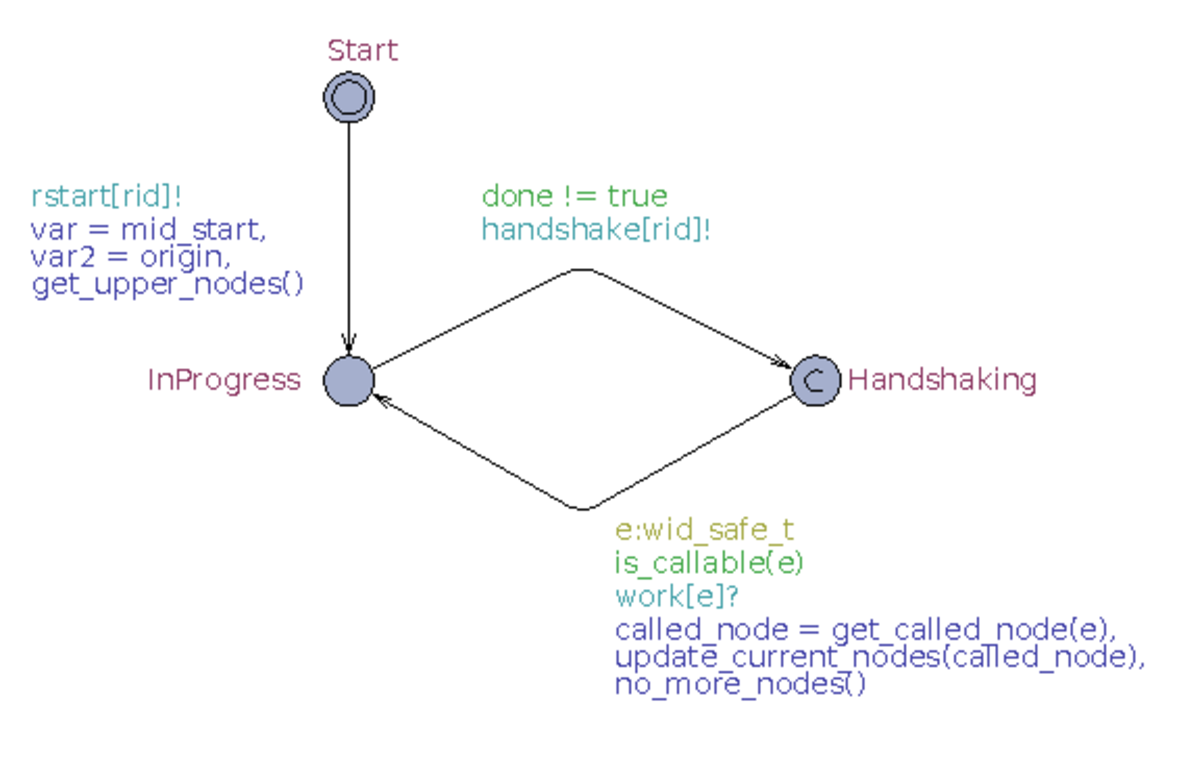
\includegraphics[width=\textwidth]{recipe.pdf}
\caption{Recipe template}
\label{fig:recipe}
\end{figure}

Having all recipe instances compete for a place on the factory leads to a large state-space, when we ask UPPAAL to find the best timed trace. In order to get around this we enforce a certain order in which recipes may be placed into the factory.  This is done using a queuing system, which we implement using the \emph{RecipeQueue} template as seen in \cref{fig:recipequeue}.

The template is instantiated with an array of recipe id's indicating the order in which we wish the recipes produced. Once instantiated, the queue may have a recipe dequeued, which may then begin processing. This reduces the state space, as recipes are to begin in a specified order. We will not get into how to produce an efficient ordering of recipes here, as it will be brought up in \cref{ch:configuration}.

\begin{figure}[h]
\centering
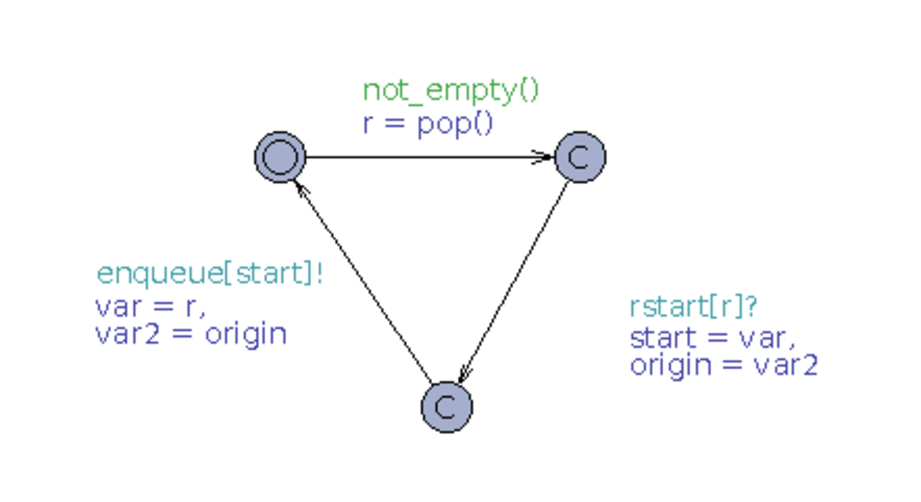
\includegraphics[width=\textwidth]{recipequeue.pdf}
\caption{RecipeQueue template}
\label{fig:recipequeue}
\end{figure}